\section{\method{}: Building Shared Decision Landscapes}
\label{sec:method}

\begin{figure*}[t]
\centering
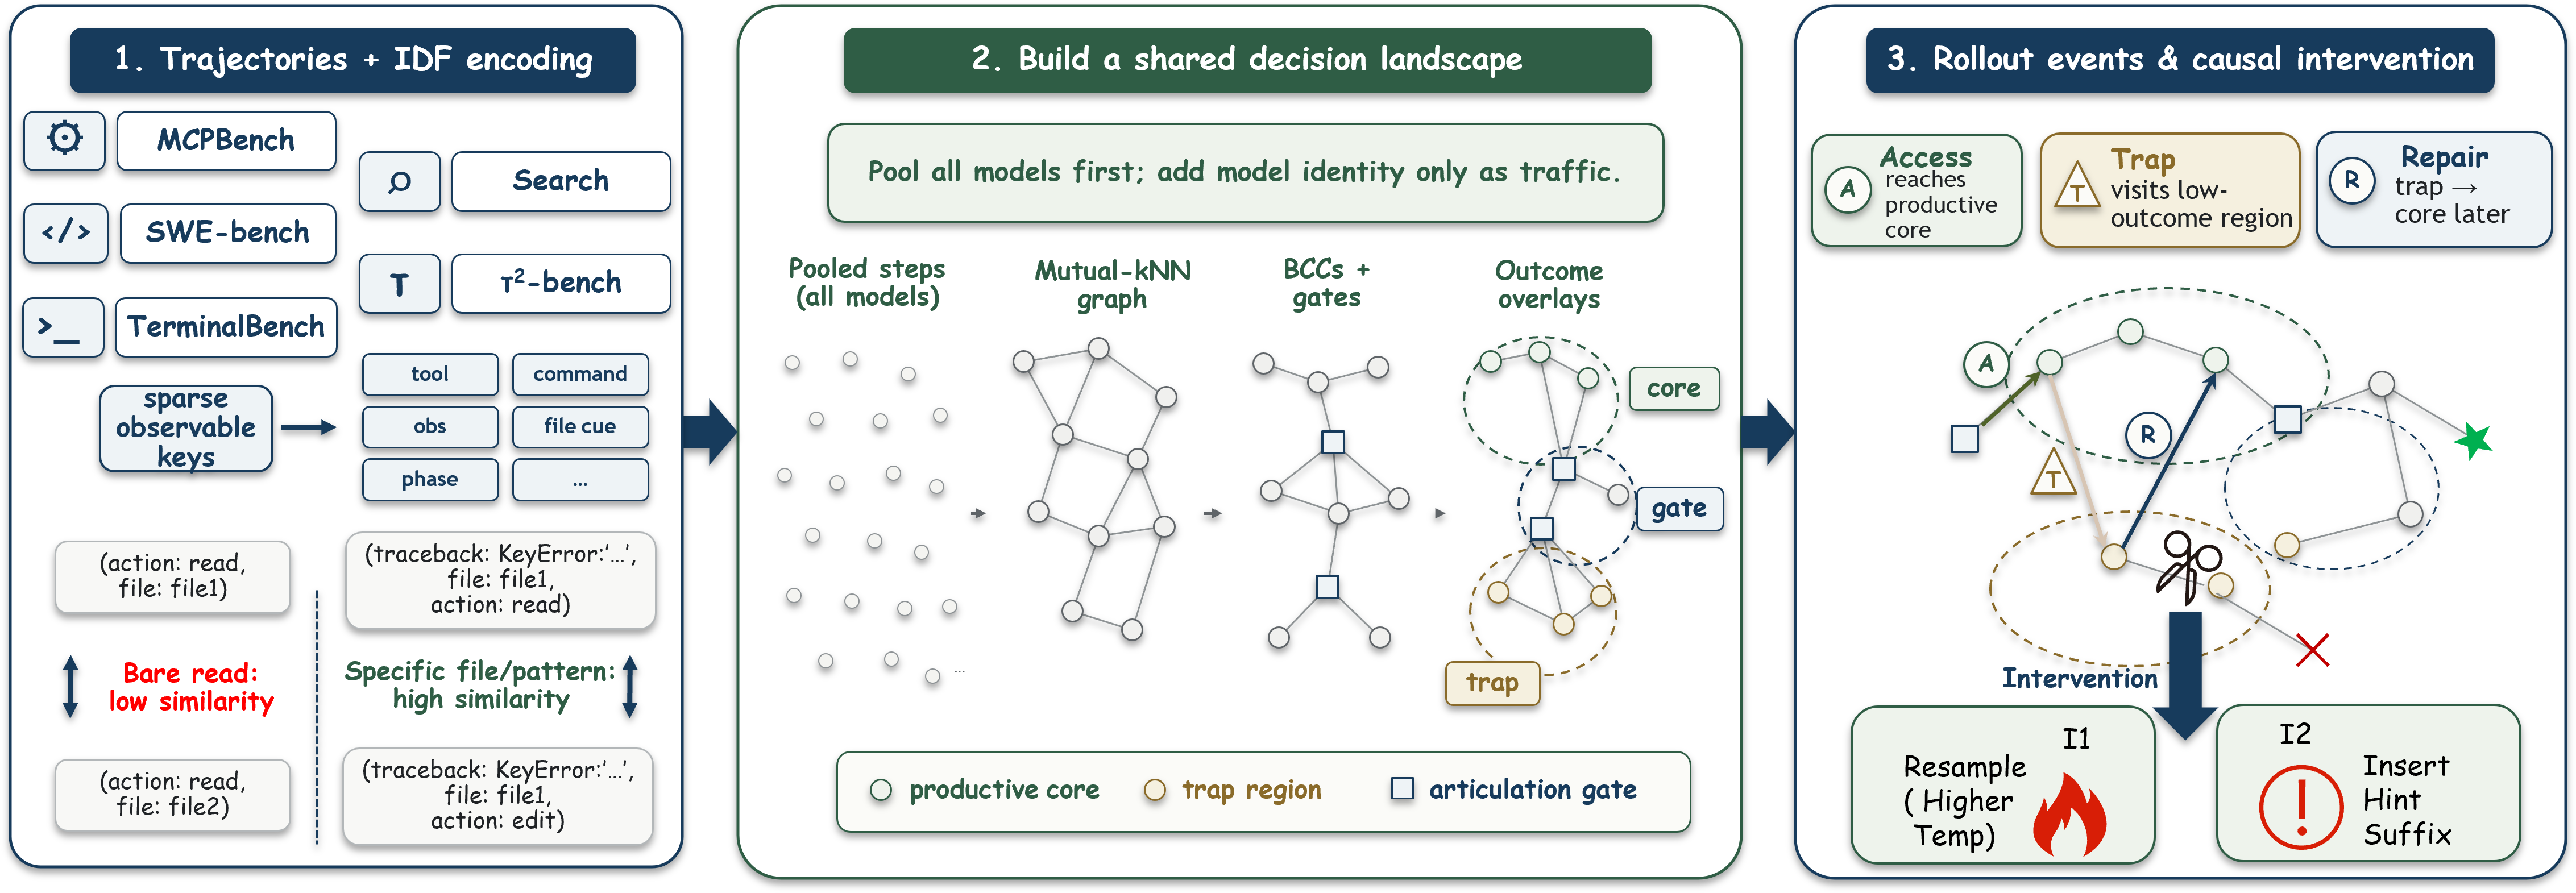
\includegraphics[width=\textwidth]{figures/pipeline.png}
\caption{Overview of \method{}. \textbf{Stage~1}: action--observation steps from five benchmark splits are encoded into sparse observable keys and compared via IDF-weighted Jaccard similarity. \textbf{Stage~2}: all model rollouts are pooled into a mutual-$k$NN graph, decomposed into BCCs and articulation gates, then annotated with outcome-informed overlays (productive cores, trap regions). \textbf{Stage~3}: three rollout events---Access, Trap, and Repair---are read from each model's path. The same trap overlay later seeds a runtime trigger for a lightweight \swe{} recovery pipeline.}
\label{fig:pipeline}
\end{figure*}

\method{} takes as input a set of agent rollouts and returns a shared decision landscape with three readable rollout events.
For a task $t$, let $\mathcal{R}_t=\bigcup_m\mathcal{R}_{t,m}$ be all rollouts from all available models.
Because the released data contain only a few passes per model per task, \method{} builds one landscape from $\mathcal{R}_t$ and compares models only after that landscape is fixed.
This separation is central to the framework: graph construction defines the terrain, while model and benchmark analyses are overlays on that terrain.

\subsection{Stage 1: Building the Shared Landscape}
\label{sec:shared_graph}

Each action--observation step $i$ is encoded as a sparse set of observable keys $K_i$: tool and action type, command class, observation pattern, file cue, temporal phase, and a pre-specified search-interaction family for \searchb{}.
Pairwise similarity is IDF-weighted Jaccard overlap over key sets,
\begin{equation}
\mathrm{sim}(i,j)=\frac{\sum_{k\in K_i\cap K_j}\idf(k)}{\sum_{k\in K_i\cup K_j}\idf(k)},
\label{eq:sim}
\end{equation}
so rare and more informative keys like a specific traceback pattern at a specific file weigh more than generic ones like a bare ''read'' action.
We convert this to a distance $d(i,j)=1-\mathrm{sim}(i,j)$; among mutual-$k$NN pairs, the graph edge weight is $w_{ij}=\exp(-d(i,j)/\sigma)$ with fixed scale $\sigma$.
For each task we build this mutual-$k$NN graph over all pooled steps, then decompose it into biconnected components (BCCs) and articulation points.
The BCC decomposition is the structural foundation of the landscape: each BCC groups steps that share dense mutual similarity, and the \emph{articulation points} (or \emph{gates}) between BCCs mark strategy or phase transitions---places where a rollout can branch into qualitatively different continuations.
A separate annotation pass confirms that 82 of 100 graph-identified articulation crossings correspond to a human-judged strategy or phase change ($4.6\times$ enrichment over random consecutive steps; see \S\ref{sec:rq1}).
Model identity is never part of the signature, distance, or graph construction.
The exact key alphabet and fixed graph hyperparameters are in Appendix~\ref{app:keys} and Appendix~\ref{tab:hyperparams_full}.

\subsection{Stage 2: Outcome Overlays}
\label{sec:overlays}

On top of the fixed BCC structure, we add two outcome-informed overlays.
Let $G_B=(\mathcal{B}_t,E_B)$ be the block quotient graph, whose nodes are BCC blocks.
For a block $b$, let $\mathcal{R}_b=\{r:\,b\in V_r\}$ be the rollouts that visit it and let $y_r\in[0,1]$ be the terminal outcome (binary for all benchmarks except the max-normalized \mcp{} reward).
We assign each block a Laplace-smoothed reward,
\begin{equation}
\hat\mu_b=\frac{\sum_{r\in\mathcal{R}_b} y_r + \tfrac{1}{2}}{|\mathcal{R}_b|+1},
\qquad
s_b=\hat\mu_b-\bar y_t,
\label{eq:block_reward_main}
\end{equation}
where $\bar y_t$ is the mean outcome over rollouts of task $t$.
To avoid treating each block independently, we diffuse this centered reward over the quotient graph:
\begin{equation}
v^{(\ell+1)}=\alpha P_B^{\top}v^{(\ell)}+(1-\alpha)s,
\label{eq:reward_diffusion_main}
\end{equation}
where $P_B$ is the row-normalized weighted adjacency matrix of $G_B$ and $v^{(0)}=s$.
After fixed-step diffusion and $L_\infty$ normalization, the productive core and trap masks are the high positive and low negative quantiles,
\begin{align}
C_t &= \{b:\, v_b>0 \;\wedge\; v_b\ge Q^+_{.75}\}, \nonumber\\
B_t &= \{b:\, v_b<0 \;\wedge\; v_b\le Q^-_{.25}\},
\label{eq:core_trap_main}
\end{align}
where $Q^+_{.75}$ is the 75th percentile among positive field values and $Q^-_{.25}$ is the 25th percentile among negative field values.
These overlays are descriptive: they locate where high- and low-outcome traffic concentrates, rather than predicting outcomes for unseen runs.
Thus $C_t$ and $B_t$ are not semantic labels like ``good action'' or ``bad action''; a trap block can still contain exploratory traffic (see \S\ref{sec:rq1}).

\subsection{Stage 3: Rollout Events}
\label{sec:profiles}

The final \method{} representation uses only three rollout events, all defined on core/trap overlays.
For a rollout $r$, let $V_r$ be its visited block set and $b_{r,1:T_r}$ its compact block sequence.
\emph{Access} asks whether $V_r$ intersects $C_t$.
\emph{Trap exposure} asks whether $V_r$ intersects $B_t$.
\emph{Repair} asks whether the sequence visits a trap and later reaches a core.
\begin{align}
A_r &= \mathbf{1}[V_r\cap C_t\ne\emptyset], \nonumber\\
E_r &= \mathbf{1}[V_r\cap B_t\ne\emptyset], \nonumber\\
R_r &= \mathbf{1}[\exists s<u:\, b_{r,s}\in B_t,\ b_{r,u}\in C_t]. \label{eq:events_main}
\end{align}
For binary-reward benchmarks, the rollout outcome is the recorded binary success/reward field; for \mcp{}, it is the per-task max-normalized continuous reward.
Appendix~\ref{app:rollout_events} gives full definitions.

\subsection{Supply and Demand Profiles}
\label{sec:supply_demand}

\method{} turns the three events into two descriptive summaries.
A model's \emph{supply} is the task-centered mean of its rollout events,
\begin{equation}
S_{m,a}=\mathbb{E}_t\bigl[a_{m,t}-\mathbb{E}_{m'\in M_t}a_{m',t}\bigr],
\end{equation}
where $a\in\{A,E,R\}$ and $a_{m,t}$ is the average event value for model $m$ on task $t$.
A benchmark's \emph{demand} is the reward-weighted contrast between high- and low-outcome traffic,
\begin{align}
D_{b,a}
&=\frac{\sum_{r\in b} y_r a_r}{\sum_{r\in b}y_r}
 -\frac{\sum_{r\in b}(1-y_r)a_r}{\sum_{r\in b}(1-y_r)}. \label{eq:demand_main}
\end{align}
For binary rewards this is simply the mean event value among resolved rollouts minus the mean event value among failed rollouts.
For \mcp{} it is the continuous analogue using normalized reward.
We use these profiles for interpretation, not as a score-prediction model.
